%%%%%%%%%%%%%%%%%%%%%%%%%%%%%%%%%%%%%%%%%%%%%%%%%%%%%%%%%%%%%%%%%%%%%%
% Overleaf (WriteLaTeX) Example: Molecular Chemistry Presentation
%
% Source: http://www.overleaf.com
%
% In these slides we show how Overleaf can be used with standard 
% chemistry packages to easily create professional presentations.
% 
% Feel free to distribute this example, but please keep the referral
% to overleaf.com
% 
%%%%%%%%%%%%%%%%%%%%%%%%%%%%%%%%%%%%%%%%%%%%%%%%%%%%%%%%%%%%%%%%%%%%%%
% How to use Overleaf: 
%
% You edit the source code here on the left, and the preview on the
% right shows you the result within a few seconds.
%
% Bookmark this page and share the URL with your co-authors. They can
% edit at the same time!
%
% You can upload figures, bibliographies, custom classes and
% styles using the files menu.
%
% If you're new to LaTeX, the wikibook is a great place to start:
% http://en.wikibooks.org/wiki/LaTeX
%
%%%%%%%%%%%%%%%%%%%%%%%%%%%%%%%%%%%%%%%%%%%%%%%%%%%%%%%%%%%%%%%%%%%%%%

\documentclass{beamer}

% For more themes, color themes and font themes, see:
% http://deic.uab.es/~iblanes/beamer_gallery/index_by_theme.html
%
\mode<presentation>
{
  \usetheme{Madrid}       % or try default, Darmstadt, Warsaw, ...
  \usecolortheme{default} % or try albatross, beaver, crane, ...
  \usefonttheme{serif}    % or try default, structurebold, ...
  \setbeamertemplate{navigation symbols}{}
  \setbeamertemplate{caption}[numbered]
} 

\usepackage[english]{babel}
\usepackage[utf8x]{inputenc}

 \newcommand{\myfrac}[2]{%
   \setbox0\hbox{$#1$}        % put the numerator in box0
   \dimen0=\wd0               % measure box0
   \setbox1\hbox{$#2$}        % put the denominator in box1
   \dimen1=\wd1               % measure box1
   \ifdim\wd0<\wd1            % if box0 is narrower than box1
   \dfrac{\hfill#1}{#2}     % put \hfill in the numerator
   \else
   \dfrac{#1}{\hfill#2}     % otherwise put \hfill in the denominator
   \fi
  }

% On Overleaf, these lines give you sharper preview images.
% You might want to `comment them out before you export, though.
\usepackage{pgfpages}
\pgfpagesuselayout{resize to}[%
  physical paper width=8in, physical paper height=6in]

% Here's where the presentation starts, with the info for the title slide
\title{Image segmentation using CRF}
\author{Santosh K, Srikanth M}
\date{}

\begin{document}

\begin{frame}
  \titlepage
\end{frame}

% These three lines create an automatically generated table of contents.
%\begin{frame}{Outline}
%  \tableofcontents
%\end{frame}

\section{}

\begin{frame}{Overview}

\begin{itemize}
  \item Given an image, segment it into objects and label them.
  \item We follow the approach described in \cite{icml_2009}.
\end{itemize}

\begin{figure}[!hbp]
    \centering
    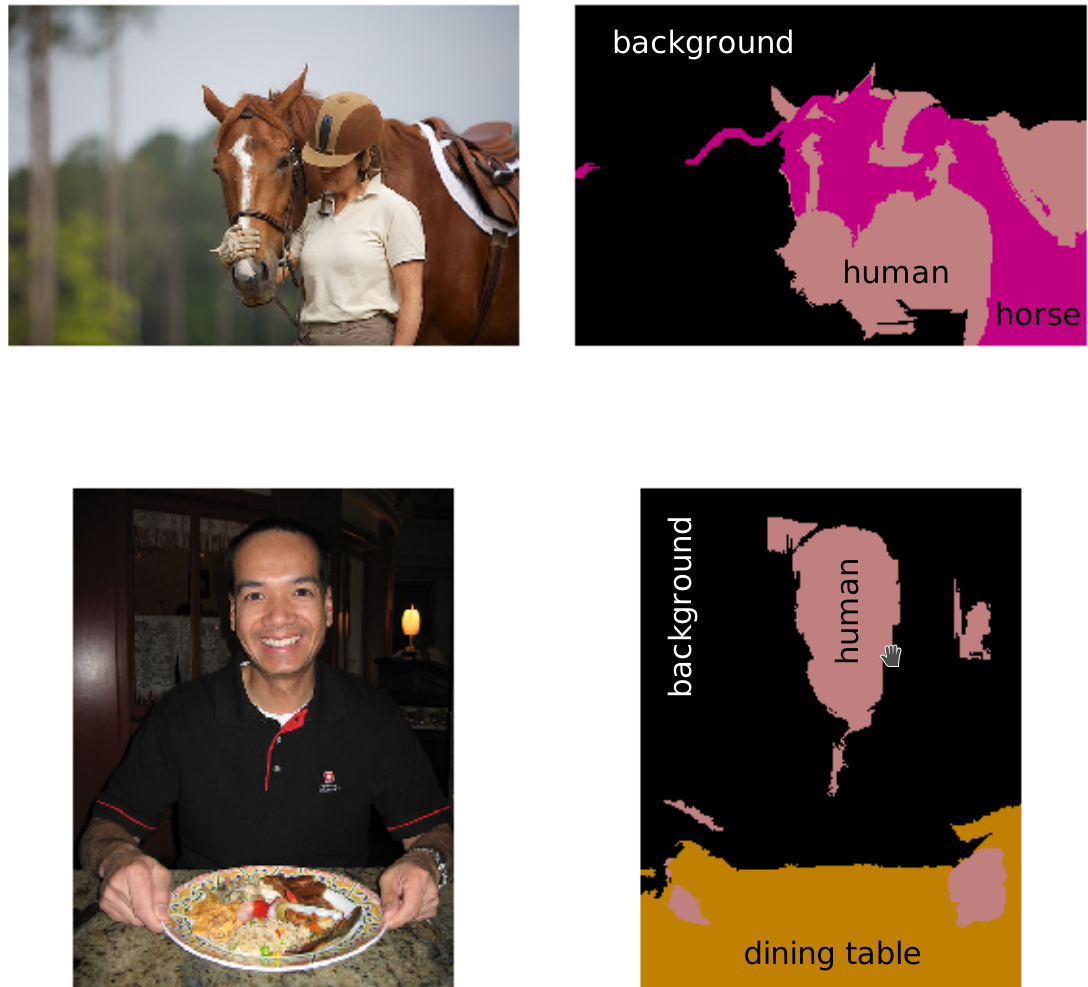
\includegraphics[width=0.5\linewidth]{images/ex}
    \caption{Sample input and segmented output images \cite{icml_2009}.}
    \label{fig_ex}
\end{figure}

\end{frame}

\begin{frame}{Approach}
  \begin{enumerate}
    \item Pre-segment the image into patches at different scales.
    \item Extract colour, texture, and SIFT features for each patch.
    \item Compute global feature vector.
    \item Use SVM to predict class of each patch.
    \item Build a CRF model, where the patch labels are dependent on each other.
    \item Apply threshold on the posteriors from the CRF to obtain final segmentation at patch level.        
  \end{enumerate}
\end{frame}

\begin{frame}{Step 1: Pre-segmentation}
    \begin{itemize}
        \item Pre-segment the image using graph cut minimization formulation \cite{Felzenszwalb:2004}.
        \item Segmentation is done at different scales (finer to coarser) by adjusting the parameters (smoothing, similarity threshold, minimum patch size) of the algorithm.        
    \end{itemize}
    \begin{figure}[!hbp]
        \centering
        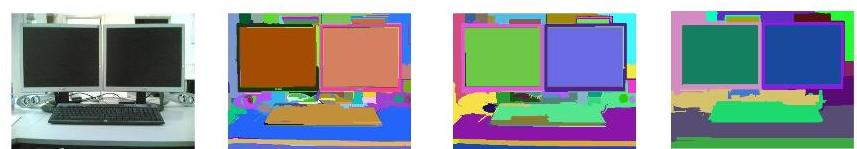
\includegraphics[width=0.9\linewidth]{images/seg_ex}
        \caption{Example pre-segmented image on different scales.}
        \label{fig_seg_ex}
    \end{figure}
\end{frame}

\begin{frame}{Step 2: Feature extraction}
  \begin{enumerate}
   \item Colour features are extracted by applying HSV transformation and computing histogram.
  \begin{enumerate}
  \item Hue and saturation are binned to 10 x 10 2D histogram.
  \item Values are binned into 10-bin histogram.
  \item Results in 110 dimension feature vector for each patch.
 \end{enumerate}
  \item Texture features using Gabor filters (we did not understand it yet).
  \item Extracted SIFT key points and descriptors for each image and used $k$-means to cluster the descriptors into 1000 clusters.
  \begin{enumerate}
      \item We compute histogram over each patch, using the VQ indices of the descriptors.
      \item Results in a 1000 dimension feature vector for each patch.
  \end{enumerate}        
  \end{enumerate}
\end{frame}

\begin{frame}{Next steps: Building CRF}
  \begin{enumerate}
    \item Class label for each patch cannot be predicted independent of other patches.
    \item Each patch is dependent on other:
    \begin{itemize}
      \item Spatial relation in the image.
      \item Overlap between patches in each scale.        
    \end{itemize}    
    \item The dependency between patches is represented with the help of a tree.
    \item Child nodes represent patch in finer level and parent node represents the patch in coarser level.    
\end{enumerate}
\end{frame}

\begin{frame}{Building CRF}
  
 \begin{figure}[!hbp]
   \centering
   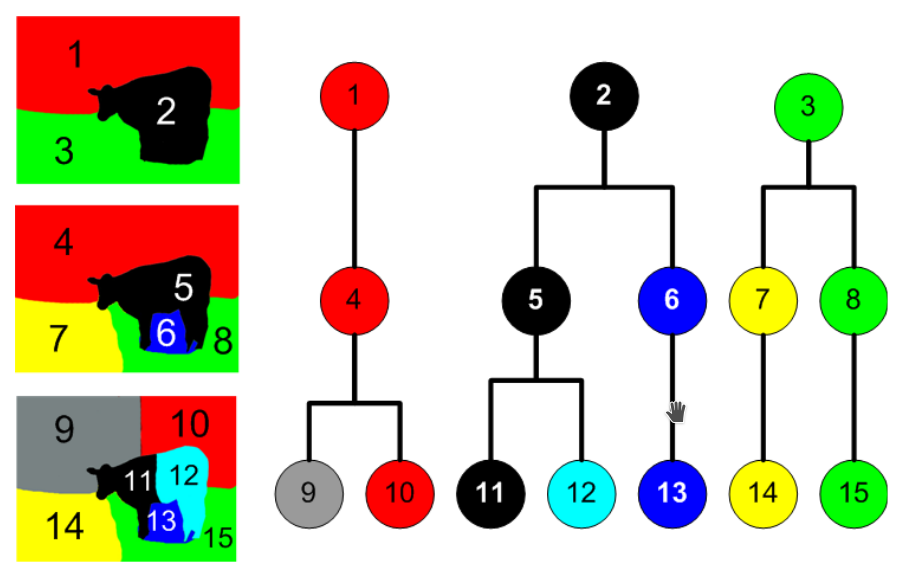
\includegraphics[width=0.9\linewidth]{images/patch_ex}
   \caption{Example of a tree built from patches at different scales \cite{Reynolds:2007}.}
   \label{fig_patch_ex}
  \end{figure}  
\end{frame}

\begin{frame}{Building CRF}
  \begin{enumerate}
    \item If $\mathbf{x}$ denotes the feature vector for a patch $p$ and $y_p$ denotes the corresponding label, then CRF for an image with $P$ patches is represented (factorized as follows:)
    \begin{equation}
    P( \mathbf{y},  \mathbf{X}) \propto \prod_{p=1}^{P} \phi(y_p, \mathbf{x}) \prod_{q \in \pi(p)}  \varphi (y_p, y_q) 
    \end{equation}
    where $\pi(p)$ denotes the child nodes of patch $p$.  
    \item The potential function $\phi$ represents local evidence for labelling patch $p$ to one the object classes $k$, and $\varphi$ represents the coupling (similarity) between patches at two different levels (parent and child from the tree).
    \item The goal is to learn the potential functions $\phi$ and $\varphi$, from the training data (images and corresponding labels with boundaries).  
  \end{enumerate}  
\end{frame}

\begin{frame}{Learning potential functions: $\phi$}
  \begin{enumerate}
    \item $\phi(y_p, \mathbf{x})$ can be obtained from a classifier (support vector machines).
    \begin{equation}
      \phi(y_p, \mathbf{x}) \propto \phi(y_p \mid \mathbf{x}, \boldsymbol{\theta}) p(\mathbf{x} \mid \boldsymbol{\theta})
    \end{equation}
    where $\boldsymbol{\theta}$ are the parameters of the classifier.
    \item SVM with $\chi^2$ kernel is observed to be good for histogram features.
    \item Further convert the output of the classifier into probabilities using $\textrm{softmax}$ function as,
    \begin{equation}
        \phi(y_p = k \mid \mathbf{x}) = \myfrac{\exp\{a_l \, \textrm{svm}(\mathbf{x}, \mathcal{C}_k) + b_l\}}{\sum_{\forall j \in K} \exp\{a_l \, \textrm{svm}(\mathbf{x}, \mathcal{C}_j) + b_l\}}
    \end{equation}
    where $l$ is the scale level, $l = \{1,2,3\}$, and $b_l$ is the scaling parameter of the $\chi^2$ kernel.
  \end{enumerate}  
\end{frame}

\begin{frame}{Learning potentials: $\varphi$}
  \begin{enumerate}
    \item The pairwise coupling or similarity between patches in two consecutive levels (i.\thinspace e., for parent $p$ at level $l$ and child $q$ at level $l+1$) is defined as,
  \begin{equation}
  \varphi(y_p, y_q) = \begin{pmatrix}
  e^{\gamma l} &   e^{-\gamma l} & \\
  e^{-\gamma l} &   e^{\gamma l} & \\
  \end{pmatrix}  
  \end{equation}
  \item Here, inference is done using junction tree algorithm (yet to understand).
  \end{enumerate}
\end{frame}

\tiny
\begin{frame}{References}
\bibliographystyle{abbrv}
\bibliography{refs}
\end{frame}
\end{document}